\documentclass[a4paper,11pt]{article}
\usepackage[american]{babel}
\usepackage[utf8]{inputenc}
\usepackage{geometry}

\usepackage{booktabs}  
\usepackage{graphicx} 
\usepackage{listings}
\lstset{%
backgroundcolor=\color{cyan!10},
basicstyle=\ttfamily,
numbers=left,numberstyle=\scriptsize
}

\usepackage[wby]{callouts}

\title{The \LaTeX-package \texttt{callouts}}
\author{Markus Stuetz}

\begin{document}

\maketitle

\section{Introduction}
In some reports or documents it may be necessary to annotate, draw arrows or put notes inside a picture. This may be done by editing the picture itself in a graphics tool or using the package TikZ. The former has the disadvantage of a different font and probably font size, the latter may require a lot of source code when using the same commands repeatedly. The package \texttt{callouts} provides a simple approach to annotate pictures.

\section{Using the package}

The package is included in the preamble as follows, with currently four pre-defined color options, listed in table \ref{tab:colors}. If no or a wrong option is specified, the package will use the default color scheme.

\begin{lstlisting}
 \usepackage[option]{callouts}
\end{lstlisting}

\begin{table}[htb]
 \centering
 \caption{Color options}\label{tab:colors}
 \begin{tabular}{cccc}
 \toprule
  option & text & background & arrow \\
  \midrule
  -& black & none & black \\
  \texttt{bwr}	& black & white & red \\
  \texttt{wby}	& white & black & yellow \\
  \texttt{bww}	& black & white & white\\
  \bottomrule
 \end{tabular}
\end{table}

Moreover, the colors for text, background, and arrow can be set directly by using the respective option keys, for instance:

\begin{lstlisting}
 \usepackage[background=gray,arrow=red]{callouts}
\end{lstlisting}

The environment itself is called \texttt{annotate} and may be put inside a \texttt{figure}-float. The environment requires two variables: The image path including a size option and the annotation scale. Make sure to put the same number in the size (e.g. \texttt{width}) option and the coordinate scale. If you decide to change the scale later on, change both numbers equally, then the relative position of the annotations will remain.

\begin{lstlisting}
 \begin{annotate}
 {\includegraphics[width=0.5\textwidth]{<file path>}}{0.5}
 \end{annotate}
\end{lstlisting}

\section{Commands for annotations}
There are currently four commands included which may follow the first two variables of the package.

\subsection{Helpgrid}
First of all, you may want to use a help grid to place your annotations. With \texttt{\textbackslash helpgrid}, a grid is drawn. The grid's coordinate origin is indicated by the dot in the center. The grid lines represent integers, coordinates are given in positive and negative decimal numbers. The default color is the background color, you may alter the color of the help grid by adding an option like so: \texttt{\textbackslash helpgrid[gray]}

\subsection{Callouts, notes, arrows }
A callout is a note, indicating to a point with an arrow. The syntax for this object is
\begin{lstlisting}
 \callout{xn,yn}{<note>}{xa,ya}
\end{lstlisting}
Here, \texttt{xn}, \texttt{yn} are the center coordinates for the note and \texttt{xa}, \texttt{ya} the coordinates for the arrow tip.

You may put a note withouth an arrow, or an arrow alone, respectively, by writing
\begin{lstlisting}
 \note{xn,yn}{<note>}
 \arrow{xs,ys}{xa,ya}
\end{lstlisting}

\newpage
\subsection{An example}
The following source code results in figure \ref{fig:Airbus}. The color option used here is \texttt{wby}. Note that the \texttt{annotate}-environment opens a \texttt{tikzpicture} environment. Hence, all TikZ-commands such as \texttt{\textbackslash draw} can be used as well, as for example in line 8.
\begin{lstlisting}
 \begin{annotate}{\includegraphics[width=0.7\textwidth]...
 ...{A319neo.jpg}}{0.7}
   % \helpgrid
   \callout{5,-3}{Engine}{1.6,-2}
   \arrow{-3,-2.4}{-4.5,-3}
   \arrow{-4.7,-3.2}{-5.5,-2.4}
   \note{1,5}{Wingtip}
   \draw [thick,\arcol] (2.5,3.8) rectangle (4,5);
 \end{annotate}
\end{lstlisting}

\begin{figure}[htb]
  \centering
  \begin{annotate}{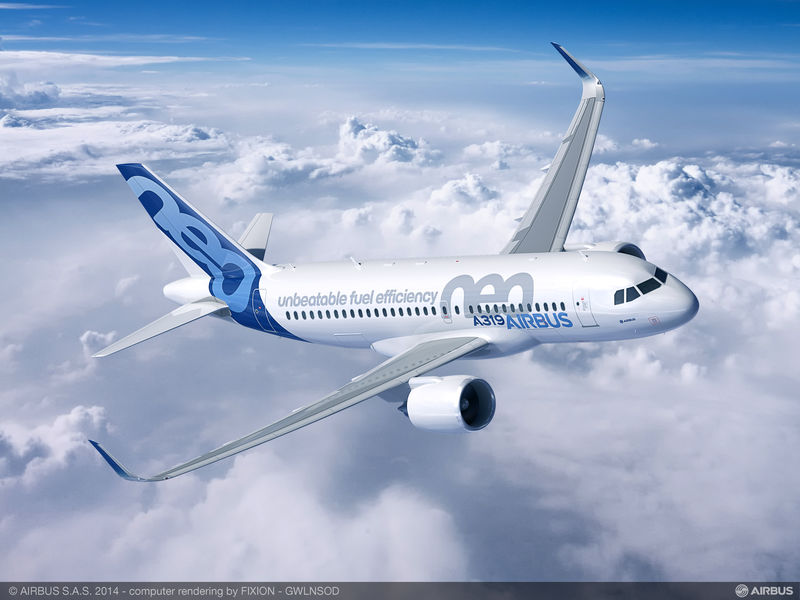
\includegraphics[width=0.7\textwidth]{A319neo.jpg}}{0.7}
%     \helpgrid
    \callout{5,-3}{Engine}{1.6,-2}
    \arrow{-3,-2.4}{-4.5,-3}
    \arrow{-4.7,-3.2}{-5.5,-2.4}
    \note{1,5}{Wingtip}
    \draw [thick,\arcol] (2.5,3.8) rectangle (4,5);
  \end{annotate}
  \caption{Airbus A319neo\protect\footnotemark}\label{fig:Airbus}
\end{figure}
 \footnotetext{Image courtesy: AIRBUS S.A.S. 2014, \texttt{www.airbus.com}, accessed 3.3.2017}
\end{document}
